\documentclass[11pt]{article}
\usepackage[margin=1in]{geometry}
\usepackage{mathpazo}
\usepackage{amsmath,amssymb}
\usepackage{microtype}
\usepackage{booktabs}
\usepackage{graphicx}
\usepackage[dvipsnames]{xcolor}
\usepackage{tikz}
\usetikzlibrary{positioning,arrows.meta,calc,fit,backgrounds,decorations.pathreplacing}
\usepackage[most]{tcolorbox}
\usepackage{enumitem}
\usepackage{listings}
\usepackage[font=small,labelfont=bf]{caption}
\usepackage{hyperref}
\hypersetup{colorlinks=true,linkcolor=MidnightBlue,citecolor=MidnightBlue,urlcolor=MidnightBlue}
\usepackage{cleveref}
\urlstyle{tt}
\def\UrlBreaks{\do\_\do/\do.}
\newcommand{\file}[1]{\nolinkurl{#1}}
\newcommand{\code}[1]{\texttt{#1}}
\newcommand{\mhh}{m_{hh}}
\newcommand{\bC}{\boldsymbol{C}}
\newcommand{\snoise}{s_{\text{noise}}}

\definecolor{trainable}{HTML}{1B6CA8}
\definecolor{physics}{HTML}{2E933C}
\definecolor{datac}{HTML}{7B4EA3}
\definecolor{warn}{HTML}{C0392B}

\newtcolorbox{keyidea}[1][]{enhanced,breakable,colback=physics!6,colframe=physics!70!black,
  fonttitle=\bfseries,title={#1},boxrule=0.6pt,arc=2pt,left=6pt,right=6pt}
\newtcolorbox{aside}[1][]{enhanced,breakable,colback=trainable!5,colframe=trainable!70!black,
  fonttitle=\bfseries,title={#1},boxrule=0.6pt,arc=2pt,left=6pt,right=6pt}
\newtcolorbox{assume}[1][]{enhanced,breakable,colback=datac!5,colframe=datac!70!black,
  fonttitle=\bfseries,title={#1},boxrule=0.6pt,arc=2pt,left=6pt,right=6pt}
\newtcolorbox{watch}[1][]{enhanced,breakable,colback=warn!5,colframe=warn!70!black,
  fonttitle=\bfseries,title={#1},boxrule=0.6pt,arc=2pt,left=6pt,right=6pt}
\setlist{itemsep=2pt,topsep=3pt}
\setlength{\emergencystretch}{3em}

\lstset{language=Python, basicstyle=\ttfamily\small, columns=fullflexible,
  keepspaces=true, commentstyle=\color{physics!70!black}\itshape,
  keywordstyle=\color{trainable!90!black}\bfseries, stringstyle=\color{datac},
  showstringspaces=false, frame=single, rulecolor=\color{gray!40},
  backgroundcolor=\color{gray!3}, xleftmargin=4pt, xrightmargin=4pt,
  aboveskip=6pt, belowskip=6pt}

\title{\textbf{The density network: results}\\[4pt]
\large Evaluated as the smooth model was, on the 1,000 test spectra}
\author{P.~Bhat (Fermilab), N.~De~Filippis (Politecnico di Bari),\\
K.F.~Johnson, H.B.~Prosper, R.~Starnes (Florida State University)}
\date{5 November 2026 (updated with the smoothness penalty)}

\begin{document}
\maketitle

\begin{keyidea}[In brief]
\begin{enumerate}
  \item \textbf{Smoothness penalty.} The fine-tuned network's poorly determined functions
    $a_{16}$--$a_{19}$ wiggled: their curvature was 10--300 times the smooth model's. A weak penalty
    on curvature ($\lambda = 10^{-6}$) removes the wiggles, leaves $a_1$--$a_{15}$ unchanged, and slightly
    \emph{improves} the accuracy. This is now the featured network.
  \item \textbf{Accuracy.} It matches the smooth model above 555~GeV ($-2\ln\lambda$ per bin 1.102
    against 1.100) and in the median per spectrum (1.073 against 1.078); below 555~GeV it is slightly
    worse (1.604 against 1.566). It is better than the old network ensemble above 555~GeV.
  \item \textbf{Calibration.} With its own model-error coefficient, determined on rows not used in
    training, its pulls have standard deviation 1.007 and are calibrated at every degree of
    cancellation. Its $\varepsilon(m)$ is the smooth model's (0.07\% at threshold, 0.28\% at 600~GeV):
    two very different models need the same model-error term.
  \item \textbf{The density} agrees with the smooth model's $d\sigma/dm$ to a median 0.31\% (0.19\% below
    555~GeV), \emph{equally at and between bin centres}; 98\% of the comparisons lie within the smooth
    model's total $\pm2\sigma$.
  \item \textbf{Below the fitted range}, both models predict the unused 240--255~GeV bin 7\% high.
\end{enumerate}
\end{keyidea}

\tableofcontents

% ===========================================================================
\section{What was evaluated}

\code{HEFTDensity} (SiLU, threshold factor, input $z \propto \sqrt{m - 250~\text{GeV}}$, 8 Gauss--Legendre
nodes per bin). The L1 starting network \file{runs/DENS_L1_SiLU_thr} and seven fine-tunes from it, all
with Poisson variances from the model and full-batch Adam (5,000 steps):
\begin{itemize}
  \item four without a penalty: Huber loss of the pulls with $\delta = 1, 2, 3$, and plain $\chi^2$
    (\file{runs/FTD_SiLU_*_pearson}, made on the 5090);
  \item three with $\delta = 2$ and the smoothness penalty, $\lambda = 10^{-6}, 10^{-5}, 10^{-4}$
    (\file{runs/FTD_SiLU_huber_d2_pearson_curv*}, made on a laptop CPU, 10 minutes each).
\end{itemize}
The featured network is $\delta = 2$, $\lambda = 10^{-6}$. The evaluation is
\file{code/heft_density_eval.ipynb} (about 5 minutes on a laptop); the plan was
\file{docs/density/density_eval_plan.pdf}.

% ===========================================================================
\section{The smoothness penalty}

Bin integrals cannot see structure inside a bin, and the coefficient functions whose monomials are
small or nearly degenerate over the sampled $\theta$ ($a_{16}$--$a_{19}$) are barely constrained by the
data. Without a penalty the network fills that freedom with small-scale wiggles. The penalty added to
the fine-tune loss is $\lambda R$, with
\begin{equation}
  R = \frac{1}{23}\sum_{i=1}^{23} R_i, \qquad
  R_i = \frac{\sum_j \big(g_i''(z_j)\big)^2}{\sum_j g_i(z_j)^2}, \qquad g_i = P_i\,e^{Q_i},
\end{equation}
the relative curvature of each function's smooth part (without the threshold factor, which is
physics), in the network's input $z = 2\sqrt{(m - 250)/1205} - 1$, on 1,201 equally spaced points. This is
the variable in which the spline model's smoothness prior acts (its knots are uniform in
$\sqrt{m - 250}$). Dividing by $\sum g_i^2$ treats functions of very different sizes alike.

\begin{table}[h]
\centering
\small
\setlength{\tabcolsep}{4pt}
\begin{tabular}{lccccccc}
\toprule
 & \multicolumn{3}{c}{$-2\ln\lambda$ per bin} & median $R_i$ & $R_i$, $i = 16 \dots 19$ & \multicolumn{2}{c}{r.m.s.\ diff.\ from smooth (\%)}\\
 & 255--555 & $>555$ & median & $a_1$--$a_{15}$ & & $a_{16}$--$a_{19}$ & $a_{20}$--$a_{23}$\\
\midrule
smooth model & 1.566 & 1.100 & 1.078 & 134 & 960, 583, 16, 426 & -- & --\\
\midrule
$\lambda = 0$ & 1.623 & 1.099 & 1.075 & 141 & 289k, 170k, 6.2k, 4.8k & 12.8 & 2.4\\
$\boldsymbol{\lambda = 10^{-6}}$ & \textbf{1.604} & \textbf{1.102} & \textbf{1.073} & 136 & 1270, 1026, 1557, 319 & 9.1 & 1.7\\
$\lambda = 10^{-5}$ & 1.612 & 1.102 & 1.076 & 120 & 315, 276, 408, 86 & 25.1 & 1.4\\
$\lambda = 10^{-4}$ & 1.665 & 1.104 & 1.090 & 102 & 56, 39, 86, 10 & 32.3 & 2.8\\
\bottomrule
\end{tabular}
\caption{The effect of the penalty ($\delta = 2$). $R_i$ as defined above (for the smooth model, of
$a_i/\phi$). The r.m.s.\ difference from the smooth model's $a_i$ is relative to $\max|a_i|$, on the $z$
grid; medians over the functions in each group.}
\label{tab:curv}
\end{table}

\begin{itemize}
  \item At $\lambda = 10^{-6}$ the curvature of $a_{16}$--$a_{19}$ falls by factors of 4--300, to the level of
    the smooth model's own, while $a_1$--$a_{15}$ are untouched (median $R_i$ 136 against 141). The accuracy
    improves slightly, and the network's $a_{16}$--$a_{19}$ move \emph{towards} the smooth model's.
  \item At $\lambda = 10^{-5}$ the network is smoother than the smooth model, and its $a_{16}$--$a_{19}$ settle on a
    different smooth solution (25\% from the smooth model's); at $10^{-4}$ even the well-determined functions
    are flattened and the accuracy suffers (1.665, 1.090).
  \item The differences that remain for $a_{16}$--$a_{19}$ (2--8\% on a 1~GeV grid for $\lambda = 10^{-6}$) are well
    within the smooth model's own uncertainties for these functions (median relative uncertainty 21--74\%,
    \file{docs/smooth/smooth_results.pdf}).
\end{itemize}

% ===========================================================================
\section{Accuracy}

For each bin, with $n$ the exact POWHEG count and $\mu$ the prediction in events, the likelihood-ratio
statistic $-2\ln\lambda = 2[\mu - n + n\ln(n/\mu)]$ has mean 1 for a correct model.

\begin{table}[h]
\centering
\small
\begin{tabular}{lccccc}
\toprule
 & \multicolumn{2}{c}{mean $-2\ln\lambda$ per bin} & median & spectra & predictions\\
model & 255--555 GeV & $>555$ GeV & per spectrum & with mean $>5$ & $\le 0$\\
\midrule
smooth model & 1.566 & 1.100 & 1.078 & 4 & 0\\
free fit per bin (the floor) & 1.559 & 1.105 & 1.075 & 4 & 0\\
old network ensemble & 1.561 & 1.121 & 1.085 & 3 & 3\\
\midrule
density, L1 (start) & 2.849 & 1.199 & 1.137 & 22 & 66\\
density, Huber $\delta = 1$ & 1.635 & 1.098 & 1.074 & 5 & 1\\
density, Huber $\delta = 2$ & 1.623 & 1.099 & 1.075 & 4 & 1\\
density, Huber $\delta = 3$ & 1.610 & 1.103 & 1.077 & 4 & 1\\
density, $\chi^2$ & 1.579 & 1.106 & 1.082 & 5 & 2\\
\textbf{density, $\delta = 2$, $\lambda = 10^{-6}$} & \textbf{1.604} & \textbf{1.102} & \textbf{1.073} & 4 & 1\\
\bottomrule
\end{tabular}
\caption{Accuracy on the 1,000 test spectra (80,000 bins).}
\label{tab:acc}
\end{table}

\begin{figure}[h]
\centering
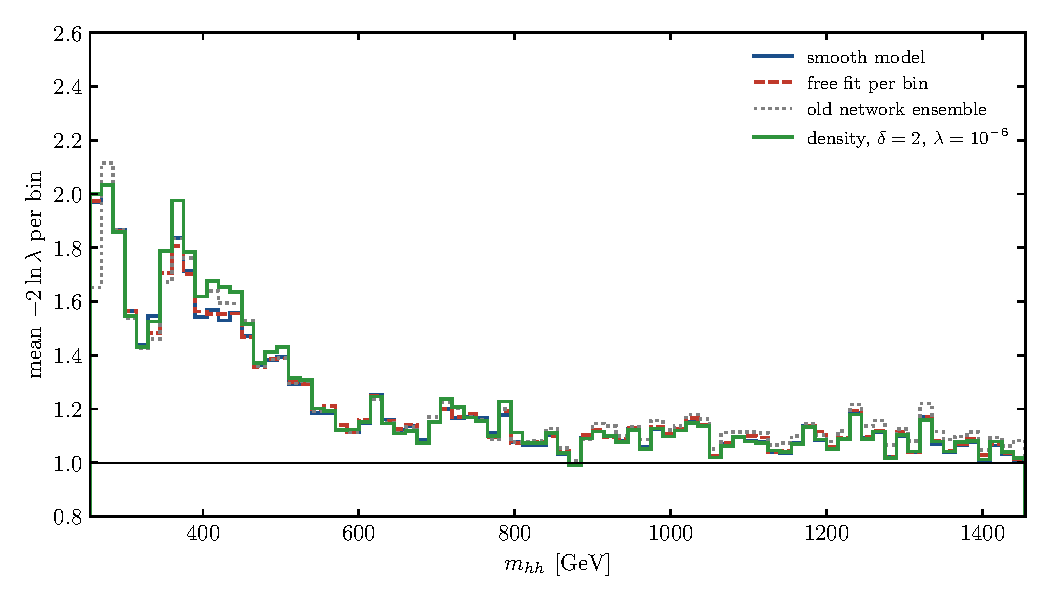
\includegraphics[width=0.7\textwidth]{fig_eval_accuracy.pdf}
\caption{Mean $-2\ln\lambda$ per bin against $\mhh$.}
\label{fig:acc}
\end{figure}

Above 555~GeV the density network is as accurate as the smooth model and the free fit, and better than the
old ensemble (trained with weights from the observed counts, and biased low there). Below 555~GeV the
fine-tunes are 0.01--0.07 above the smooth model; the smaller the Huber $\delta$, the less the fit is driven
by the large pulls of the most cancelling spectra, and the larger the mean. The difference is small next to
the common excess over 1 (the systematic of \file{docs/dihiggs_model.pdf}, section 6), and these are single
seeds. The fine-tune is essential: the L1 starting network is far from the floor near threshold.

\begin{aside}[Why the fine-tune notebook gives different numbers]
\file{heft_finetune.ipynb} reports Neyman's $\chi^2$, $(n-\mu)^2/n$, with $n$ estimated from $N_\text{eff}$. Using
the observed count as the variance favours predictions that are biased low, and the density networks,
fitted with their own Poisson variances, are not. The likelihood-ratio statistic has no such preference,
which is why the paper uses it.
\end{aside}

% ===========================================================================
\section{Calibration}

Each model gets its own model-error coefficient $\varepsilon(m)$, determined on the 38,076 quick-test rows (never
used in training) by requiring unit variance of the pulls in each bin, then smoothing $\ln\varepsilon$ by a
quadratic. The network has no fit uncertainty; it is set to zero.

\begin{table}[h]
\centering
\small
\setlength{\tabcolsep}{4pt}
\begin{tabular}{lccccc}
\toprule
 & \multicolumn{3}{c}{s.d.\ of the pull} & & $\langle z^2\rangle$ by cancellation fifth\\
model, model-error term & all & 255--555 & $>555$ & $|z|<2$ & (1 = strongest \dots\ 5)\\
\midrule
smooth model, own $\varepsilon$ & 1.004 & 1.011 & 1.001 & 95.4\% & 0.97, 0.98, 1.04, 1.04, 1.00\\
smooth model, none & 1.090 & 1.218 & 1.043 & 93.9\% & 1.70, 1.10, 1.07, 1.06, 1.01\\
\midrule
density (featured), own $\varepsilon$ & 1.007 & 1.015 & 1.005 & 95.4\% & 1.00, 0.99, 1.04, 1.04, 1.00\\
density (featured), smooth model's $\varepsilon$ & 1.003 & 1.008 & 1.001 & 95.5\% & 0.98, 0.98, 1.03, 1.04, 1.00\\
density (featured), none & 1.104 & 1.266 & 1.044 & 93.9\% & 1.83, 1.13, 1.07, 1.05, 1.01\\
\bottomrule
\end{tabular}
\caption{Pulls on the test spectra. For a standard normal, $|z|<2$ holds for 95.4\%. All the other fine-tunes
give 1.007--1.008 with their own $\varepsilon$.}
\label{tab:cal}
\end{table}

\begin{figure}[h]
\centering
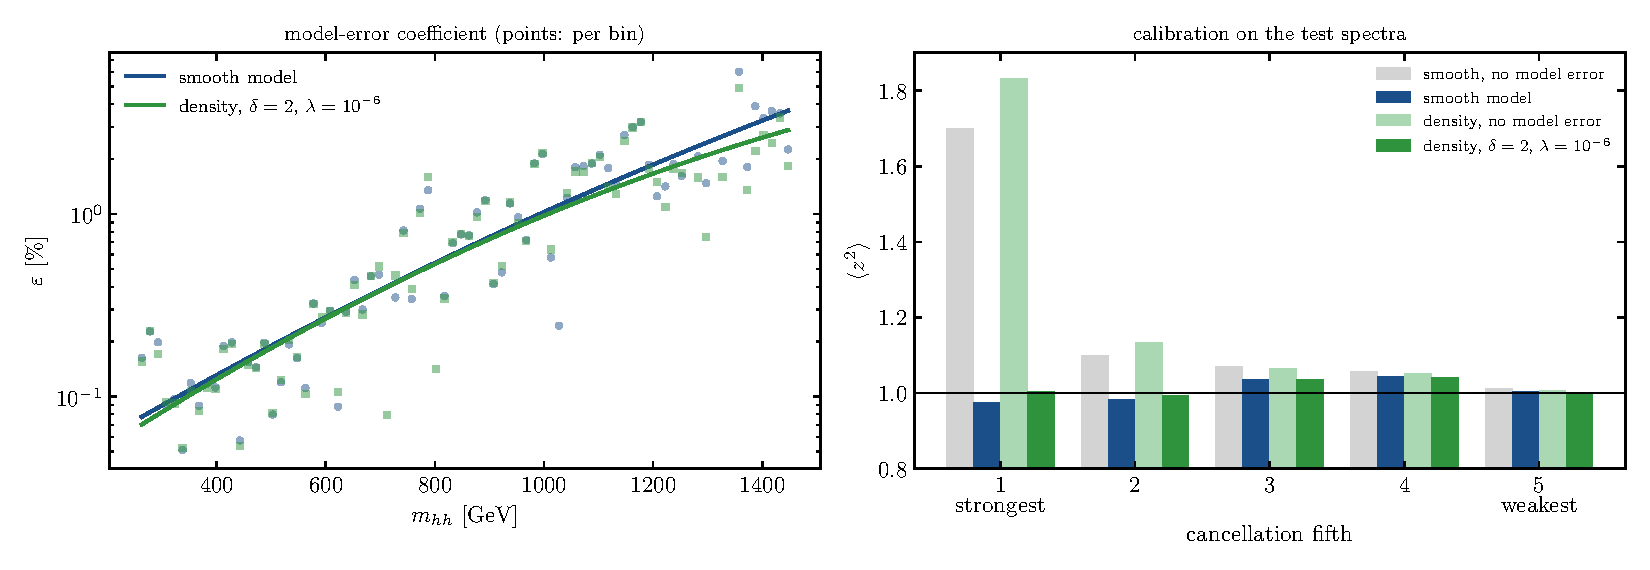
\includegraphics[width=\textwidth]{fig_eval_calibration.pdf}
\caption{Left: the model-error coefficient of the smooth model and of the featured density network (points:
per bin; lines: the smooth quadratic form). Right: $\langle z^2\rangle$ by fifth of cancellation, with and
without the model-error term.}
\label{fig:cal}
\end{figure}

The two models' $\varepsilon(m)$ agree from threshold to about 1~TeV (0.070\% and 0.077\% at 262~GeV; 0.275\% and
0.279\% at 600~GeV), and the smooth model's $\varepsilon$ calibrates the network as well as its own. Two models built
in entirely different ways need the same model-error term: the systematic is a property of the POWHEG
spectra, not of either model. Above 1~TeV the network's $\varepsilon$ is lower (2.9\% against 3.7\% at 1.45~TeV),
where both are determined from bins of about 20 events.

% ===========================================================================
\section{The density}

\paragraph{Against the smooth model.} On a 0.5~GeV grid from 255 to 1455~GeV, at the 1,000 test points:

\begin{center}
\small
\begin{tabular}{lccccc}
\toprule
 & \multicolumn{3}{c}{median $|$network $-$ smooth$|$ / smooth} & \multicolumn{2}{c}{within the smooth model's total} \\
run & all & at centres & between & $\pm1\sigma$ & $\pm2\sigma$\\
\midrule
density, L1 (start) & 1.03\% & 1.03\% & 1.03\% & 57\% & 82\%\\
density, $\delta=2$, $\lambda = 0$ & 0.33\% & 0.32\% & 0.33\% & 90\% & 97\%\\
\textbf{density, $\delta=2$, $\lambda=10^{-6}$} & \textbf{0.31\%} & \textbf{0.30\%} & \textbf{0.32\%} & \textbf{90\%} & \textbf{98\%}\\
\bottomrule
\end{tabular}
\end{center}
Below 555~GeV, for the featured network: 0.19\%, 83\% and 95\%. The ``total'' uncertainty is the smooth model's
fit uncertainty and its model-error term at the level of the density, $\varepsilon(m)\sum_i|C_ia_i(m)|$. The columns
``at centres'' and ``between'' are equal: the density network is as reliable between bin centres as at them.

\paragraph{Between bin centres} (\cref{fig:interp}). For the two spectra of moderate cancellation in the paper's
\file{fig_interpolation}, the featured network lies within 0.6\% and 2.4\% of the smooth model below 600~GeV, and
the four unpenalised fine-tunes differ among themselves by at most 0.16\% and 0.13\%, against 4.3\% and 5.4\% for
the 20 old networks. (The four share their starting network, so their spread is a lower bound on that of a seeds
ensemble.) The third spectrum passes through zero near 330~GeV, where any relative measure blows up; in absolute
terms the curves agree.

\begin{figure}[h]
\centering
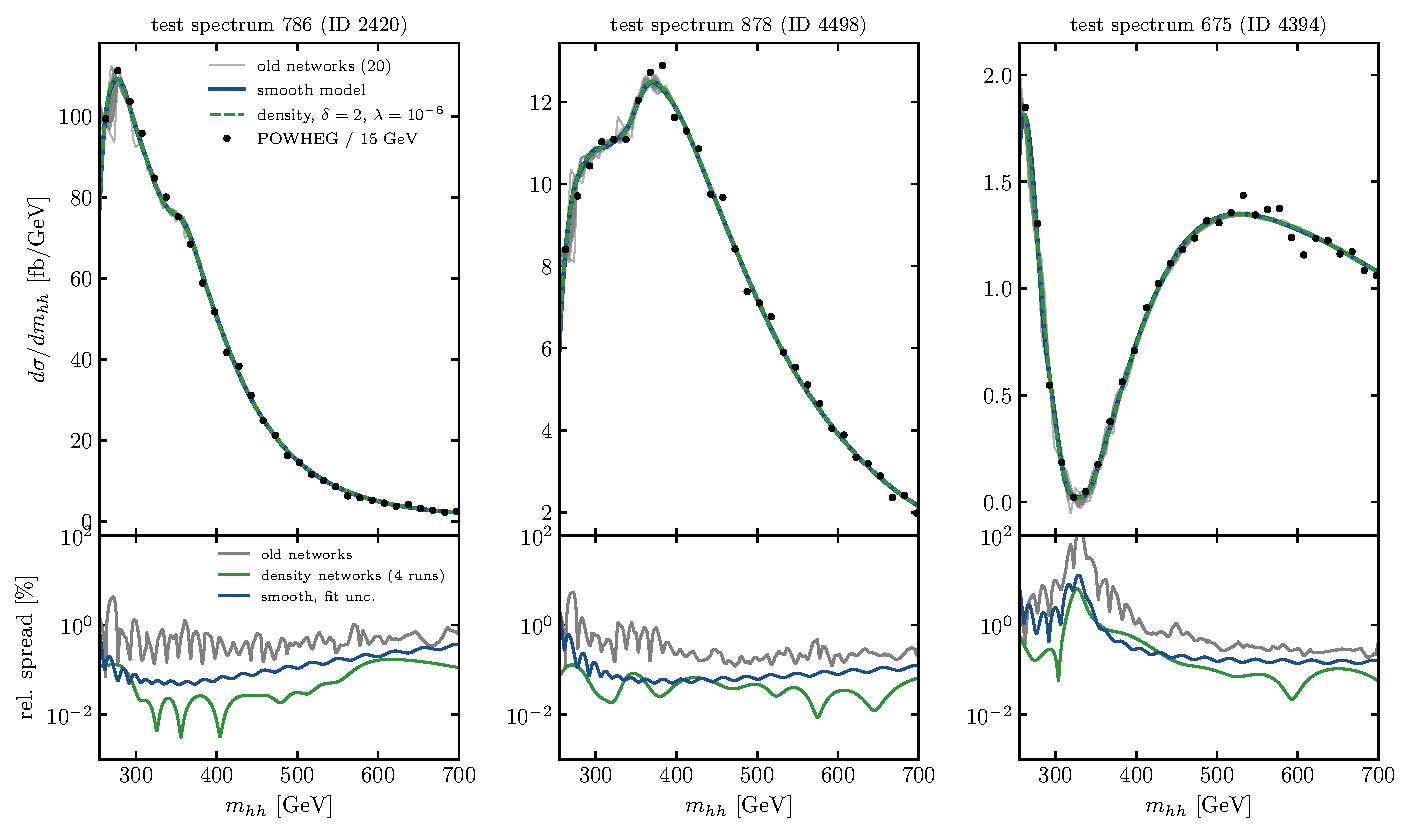
\includegraphics[width=\textwidth]{fig_eval_interpolation.pdf}
\caption{Three test spectra below 700~GeV: the 20 old networks (grey), the smooth model (blue) and the featured
density network (green, dashed), with POWHEG divided by 15~GeV. Lower panels: relative spread of the old networks
and of the four unpenalised density fine-tunes, and the smooth model's fit uncertainty.}
\label{fig:interp}
\end{figure}

\paragraph{The coefficient functions} (\cref{fig:coef}). On a 1~GeV grid, the r.m.s.\ difference between the
featured network's and the smooth model's $a_i(m)$, relative to $\max|a_i|$, is 0.04--0.5\% for $a_1$--$a_{15}$,
1.0--1.3\% for $a_{20}$--$a_{23}$, and 2--8\% for $a_{16}$--$a_{19}$. The smooth model's fit bands are very narrow (a few
per cent of the POWHEG noise), so even well-determined functions lie outside $\pm2\sigma$ over parts of the range:
the bands measure the fit uncertainty of one model, not the difference between two.

\begin{figure}[p]
\centering
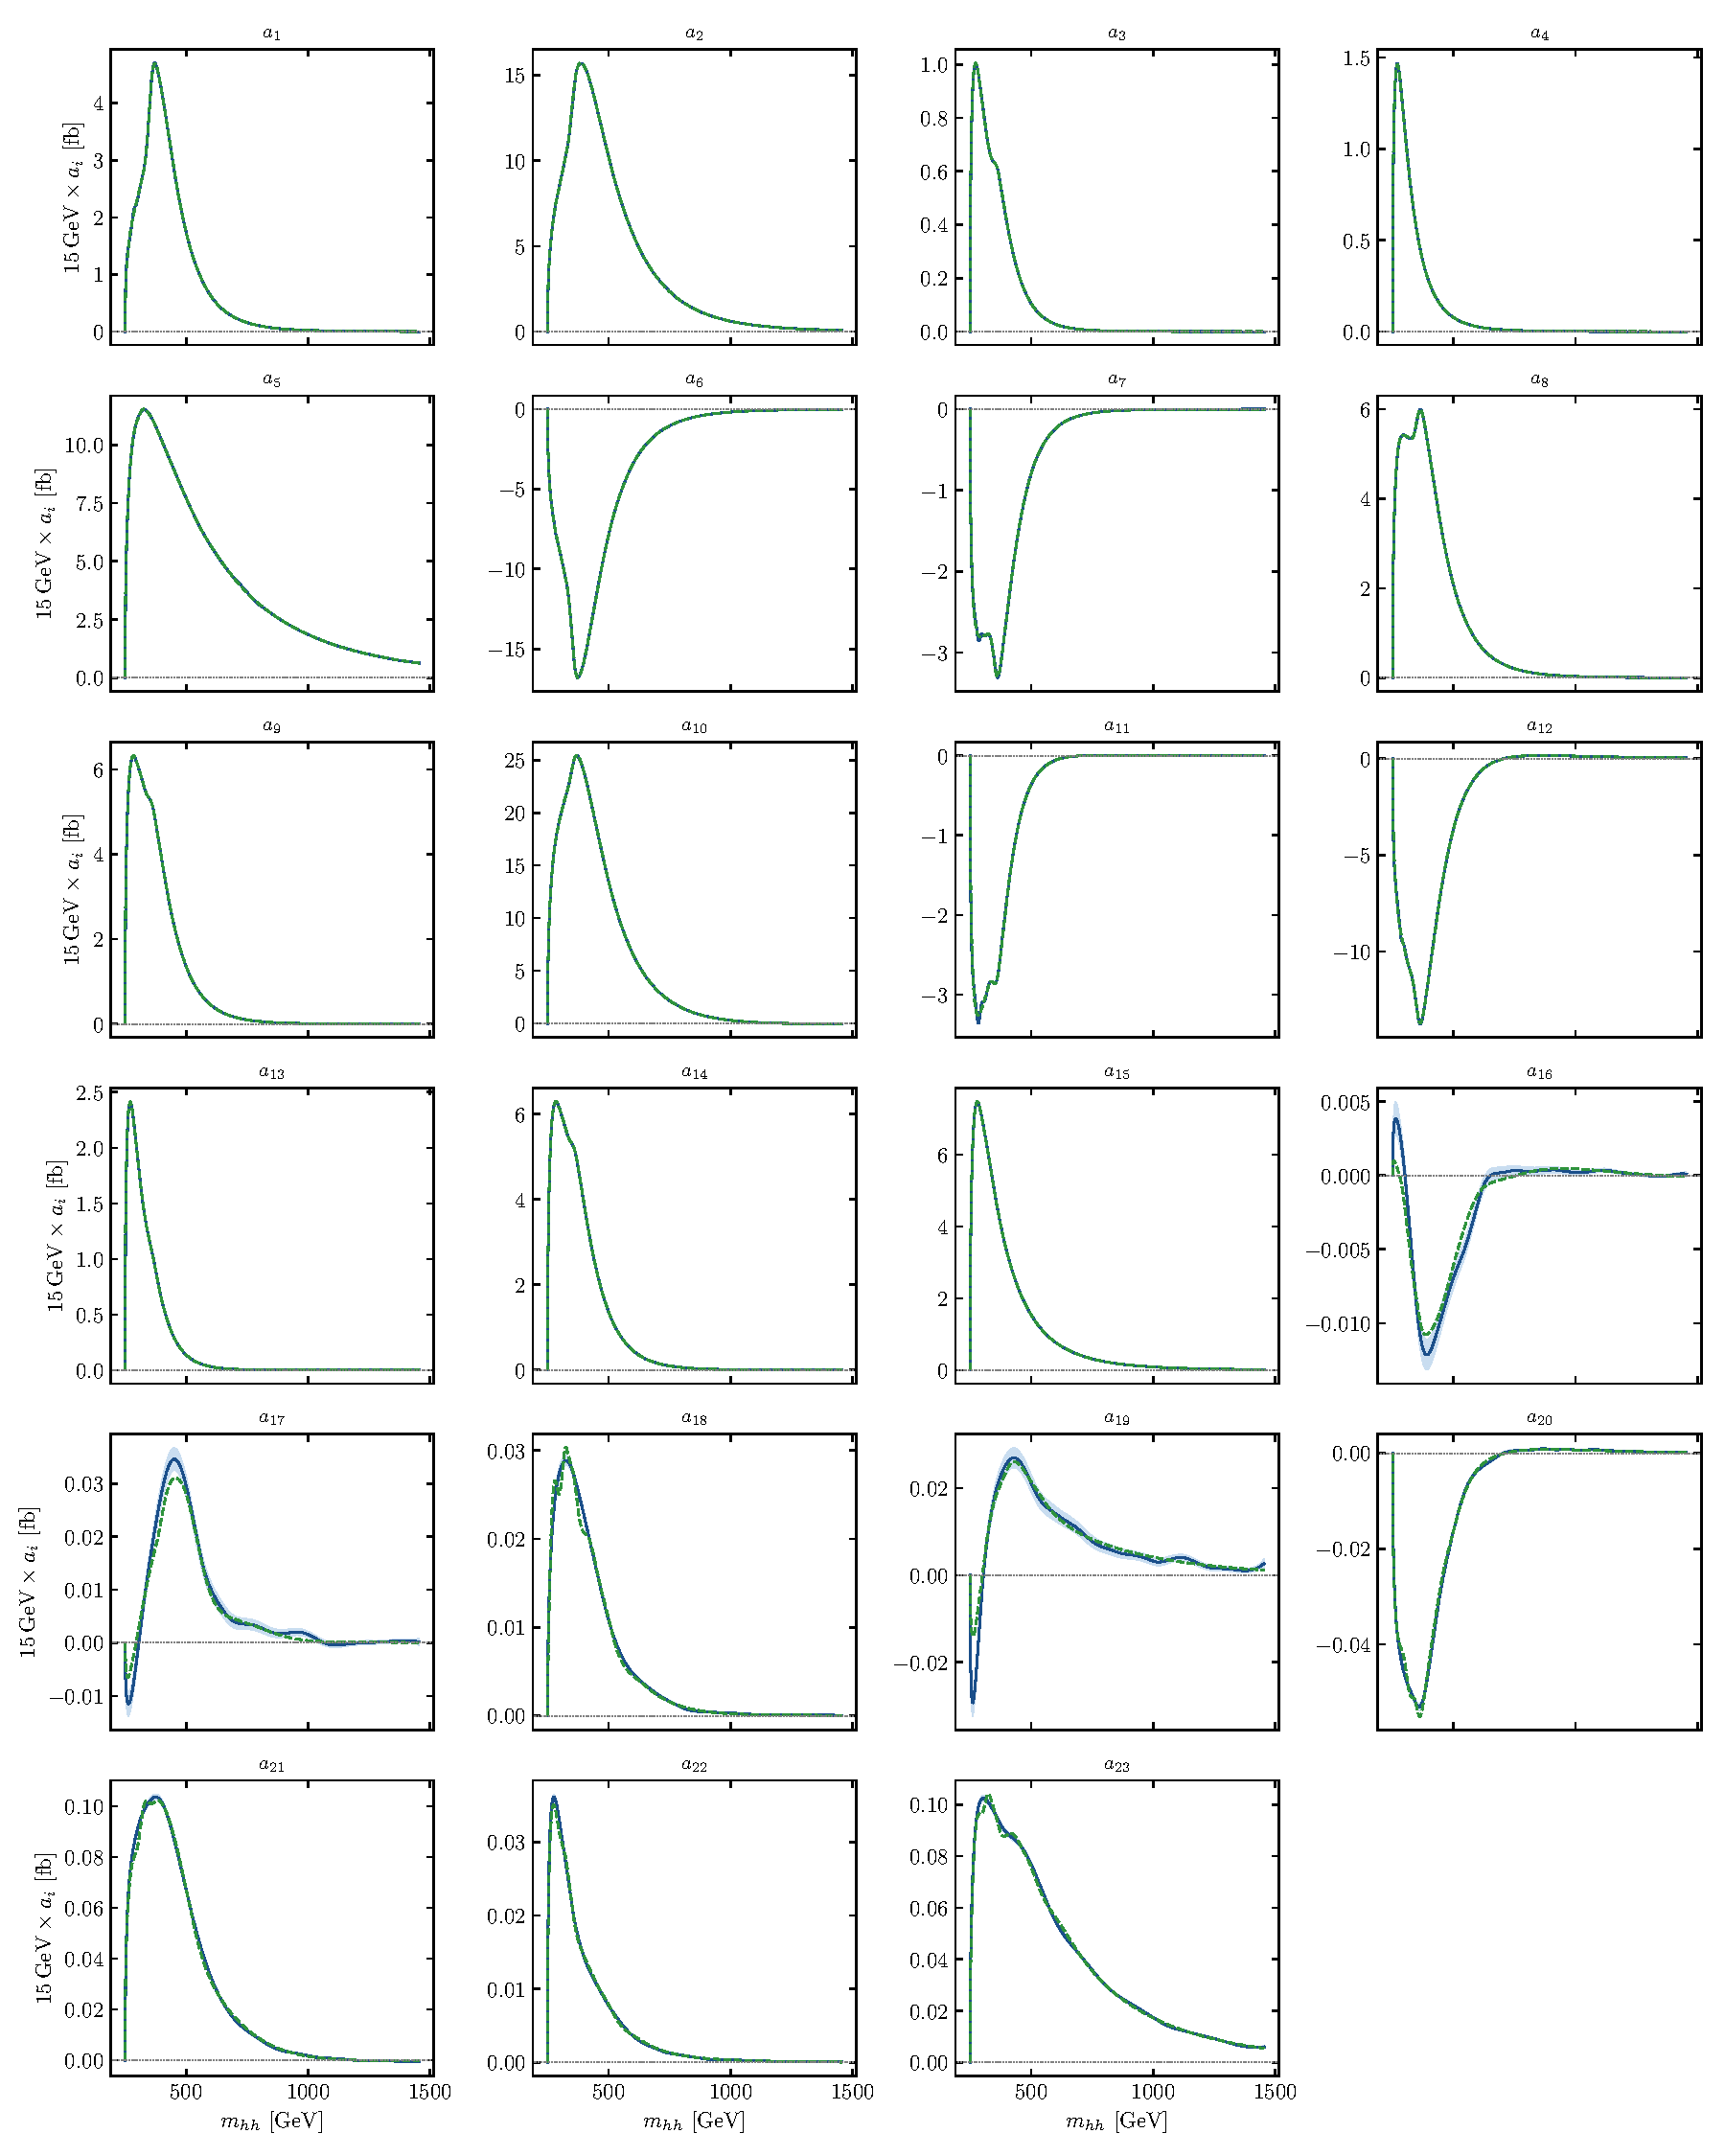
\includegraphics[width=0.9\textwidth]{fig_eval_coefficients.pdf}
\caption{The 23 coefficient functions as $15~\text{GeV}\times a_i$: smooth model with its $\pm1\sigma$ fit band (blue)
and the featured density network (green, dashed).}
\label{fig:coef}
\end{figure}

% ===========================================================================
\section{Below the fitted range}

The unused POWHEG bin 240--255~GeV holds 316,626 events over the 1,000 test spectra. With the threshold factor,
both models predict it as the integral of the density over 250--255~GeV:

\begin{center}
\small
\begin{tabular}{lcc}
\toprule
model & observed / predicted, summed & median per spectrum\\
\midrule
smooth model & 0.937 & 0.957\\
density, L1 (start) & 0.927 & 0.926\\
density, featured & 0.936 & 0.917\\
\bottomrule
\end{tabular}
\end{center}
Both over-predict the bin by about 7\%, by the same amount: the shape just above threshold, which neither sees below
255~GeV, is extrapolated the same way.

% ===========================================================================
\section{Conclusions and next steps}

\begin{itemize}
  \item With a weak smoothness penalty, the density network reaches the same floor as the smooth model, needs the
    same model-error term, and agrees with it as a density to a few tenths of a per cent, between bin centres as
    well as at them, with no wiggles. It is a genuine, independent cross-check of the paper's primary model.
  \item Near threshold it is slightly less accurate than the smooth model (1.604 against 1.566). These are single
    seeds.
  \item \textbf{Recommended settings}: Huber $\delta = 2$, $\lambda = 10^{-6}$ (\code{CURV\_LAMBDAS = [1e-6]} in
    \file{heft_finetune.ipynb}).
  \item \textbf{Next, when wanted}: a seeds ensemble of this configuration on the 5090 (fit uncertainty, spread between
    centres); the merged-bin test.
\end{itemize}

\end{document}
